%!TEX root = ../../master.tex
\chapter{Experiment: Overall Evaluation of KubeCloud and the learning activity}
\label{appendix_overall_evaluation}

\section*{Evaluation of KubeCloud}
The first part of the questionnaire consisted of questions about the cluster and the way it supported the students learning.

\subsection*{Physical appearance of the cluster}


\begin{figure}[H]%
    \centering
    \subfloat[The cluster provided me a better understanding of what a cloud consists of]{{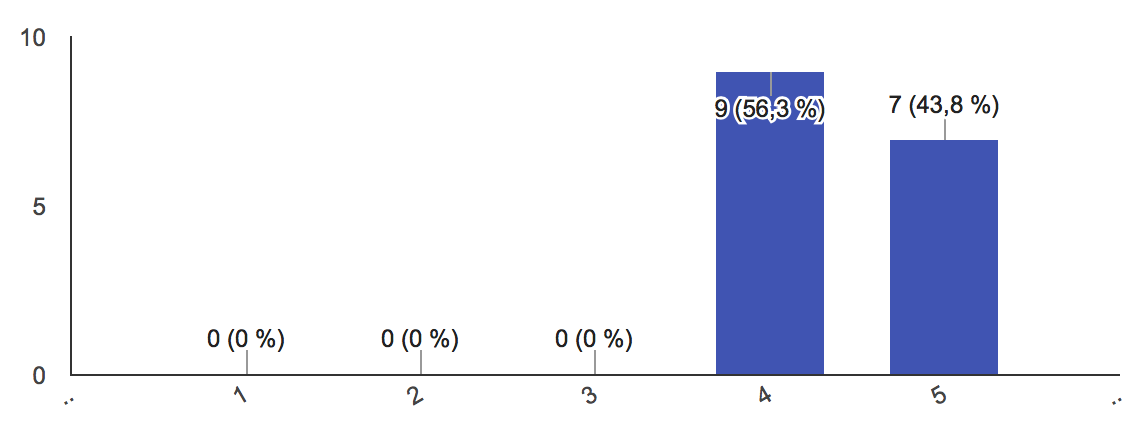
\includegraphics[width=7cm]{figures/overall_evaluation/q1_the_cluster_provided_me_a_better_understanding_of_what_a_cloud_consists_of} }}%
      \qquad
    \subfloat[The physicality of the cluster provided a better understanding of errors in distributed systems (e.g. pulling the network cable)]{{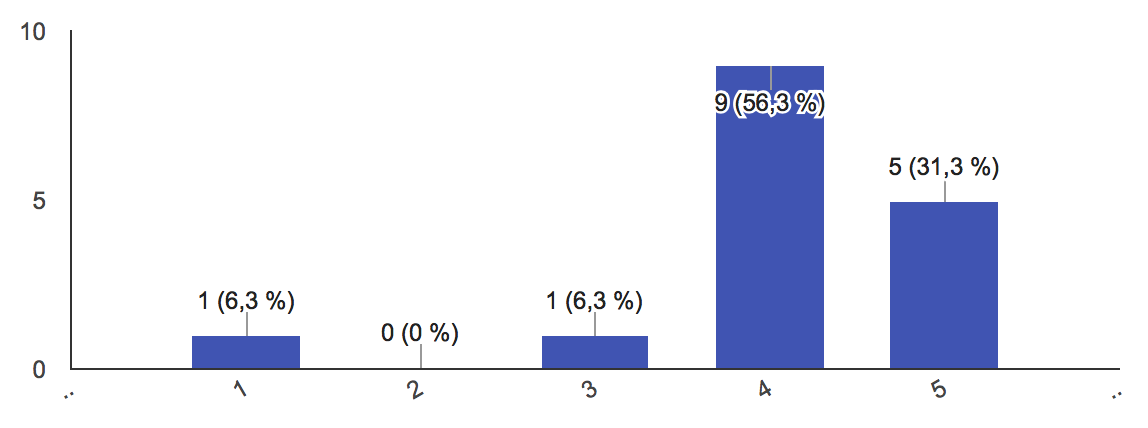
\includegraphics[width=7cm]{figures/overall_evaluation/q2_the_physicality_of_the_cluster_provided_a_better_understanding_of_errors_in_distributed_systems} }}%
          \qquad
    \subfloat[The physical design of the cluster gave me associations to a real server rack]{{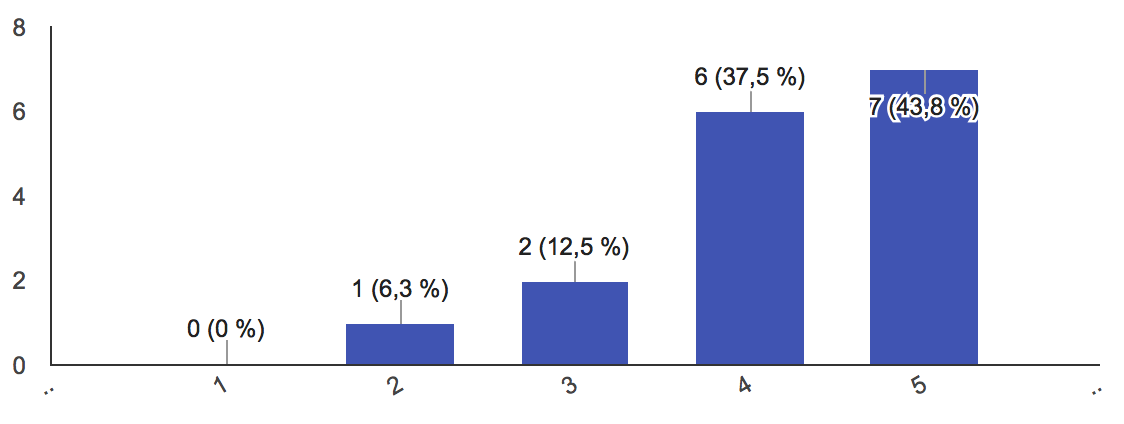
\includegraphics[width=7cm]{figures/overall_evaluation/q3_the_physical_design_of_the_cluster_gave_me_associations_to_a_real_server_rack} }}%
    \label{fig:eval_physical_appearance}%
\end{figure}

\begin{figure}[H]
    \centering
    
\includegraphics[width=\textwidth]{figures/overall_evaluation/comments_physical}
\end{figure}

\subsection*{Group activity}


\begin{figure}[H]%
    \centering
    \subfloat[The cluster allowed me to experiment]{{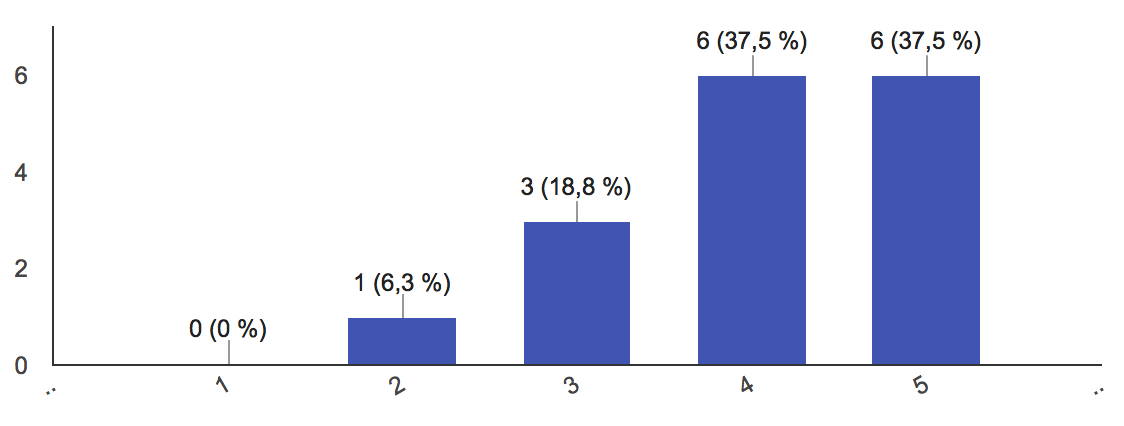
\includegraphics[width=7cm]{figures/overall_evaluation/q4_the_cluster_allowed_me_to_experiment} }}%
      \qquad
    \subfloat[The cluster initiated group discussions]{{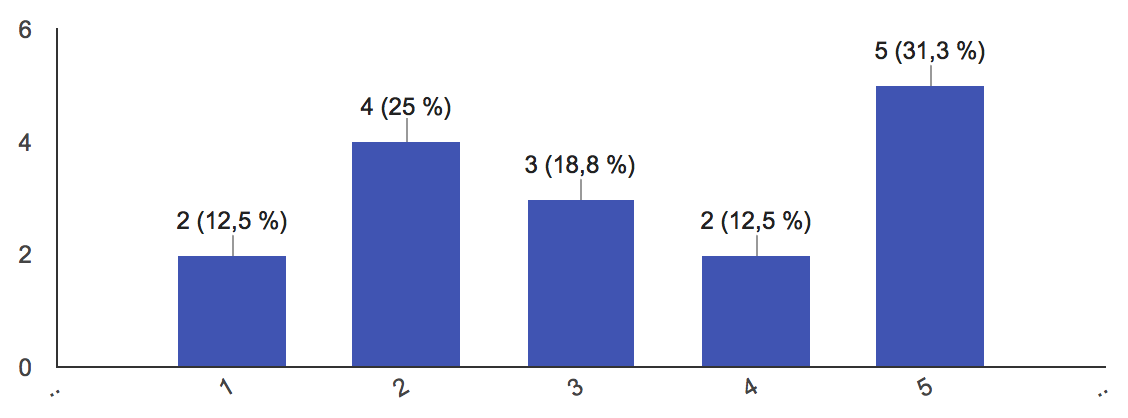
\includegraphics[width=7cm]{figures/overall_evaluation/q5_the_cluster_initiated_group_discussions} }}%
    \label{fig:eval_group_activity}%
\end{figure}


\begin{figure}[H]
    \centering
    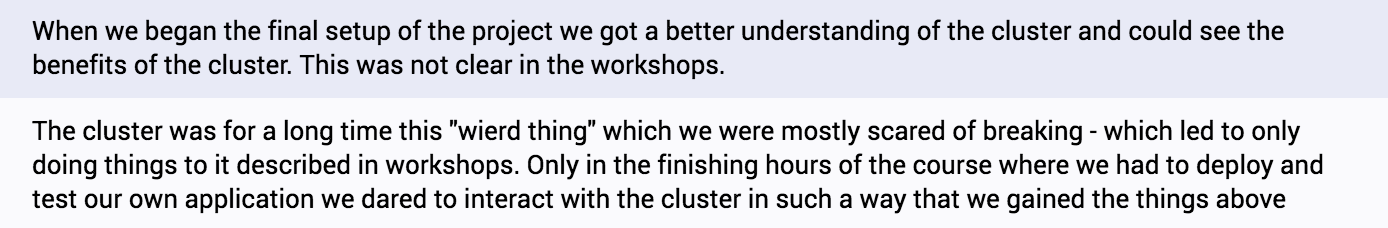
\includegraphics[width=\textwidth]{figures/overall_evaluation/comments_group}
\end{figure}

\subsection*{Visualization}


\begin{figure}[H]%
    \centering
    \subfloat[The cluster combined with the visualizer helped me understand the concepts of the cluster]{{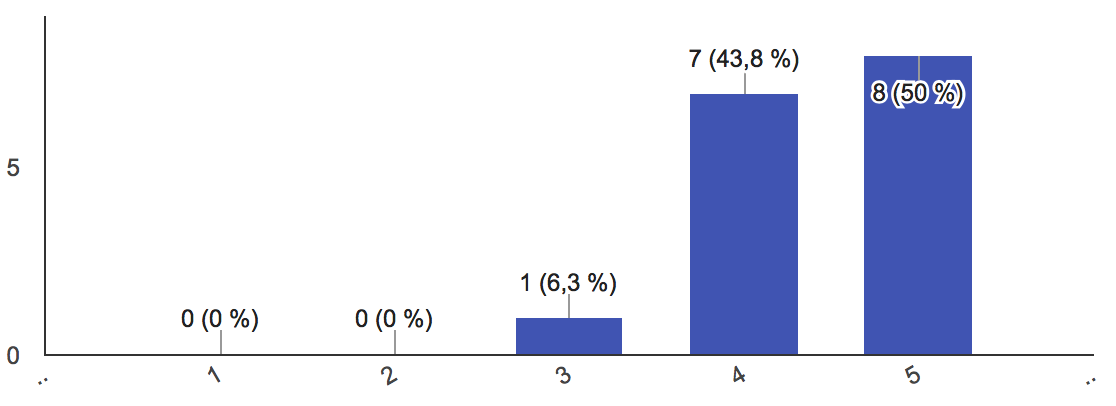
\includegraphics[width=7cm]{figures/overall_evaluation/q6_the_cluster_combined_with_the_visualizer_helped_me_understand_the_concepts_of_the_cluster} }}%
      \qquad
    \subfloat[The cluster combined with the visualizer helped me understand the how errors are handled]{{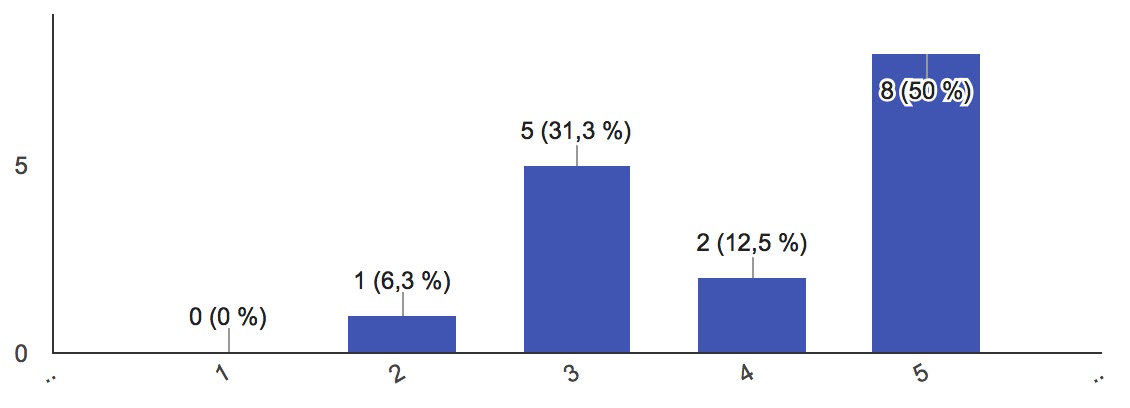
\includegraphics[width=7cm]{figures/overall_evaluation/q7_the_cluster_combined_with_the_visualizer_helped_me_understand_the_how_errors_are_handled} }}%
    \label{fig:eval_visualization}%
\end{figure}

\begin{figure}[H]
    \centering
    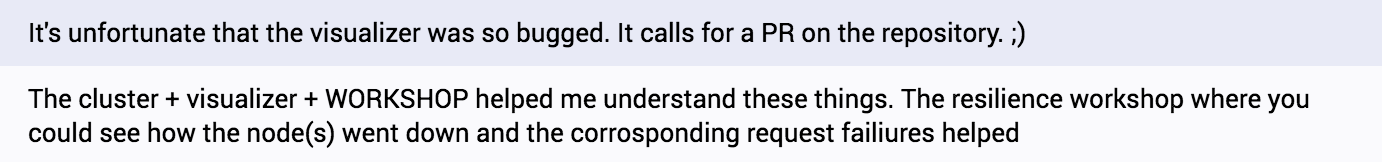
\includegraphics[width=\textwidth]{figures/overall_evaluation/comments_visualization}
\end{figure}

\newpage
\subsection*{Motivation}


\begin{figure}[H]%
    \centering
    \subfloat[The use of a cluster increased my motivation]{{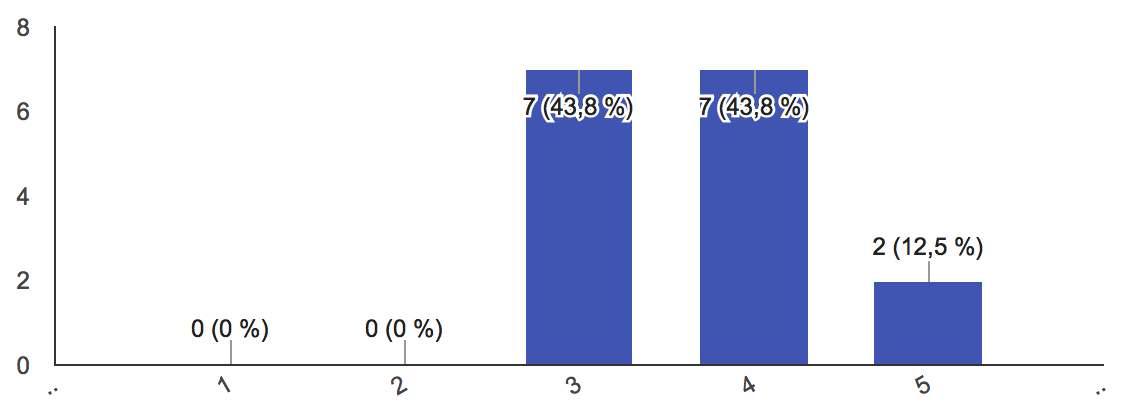
\includegraphics[width=7cm]{figures/overall_evaluation/q8_the_use_of_a_cluster_increased_my_motivation} }}%
      \qquad
    \subfloat[The cluster motivated me to do out of curriculum experimentation]{{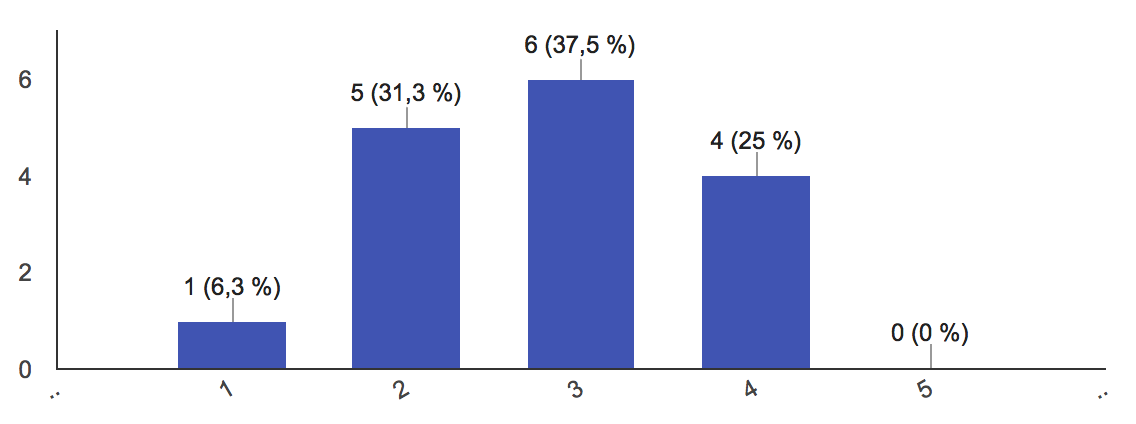
\includegraphics[width=7cm]{figures/overall_evaluation/q9_the_cluster_motivated_me_to_do_out_of_curriculum_experimentation} }}%
    \qquad
    \subfloat[The cluster was a fun and playful way of learning the concepts]{{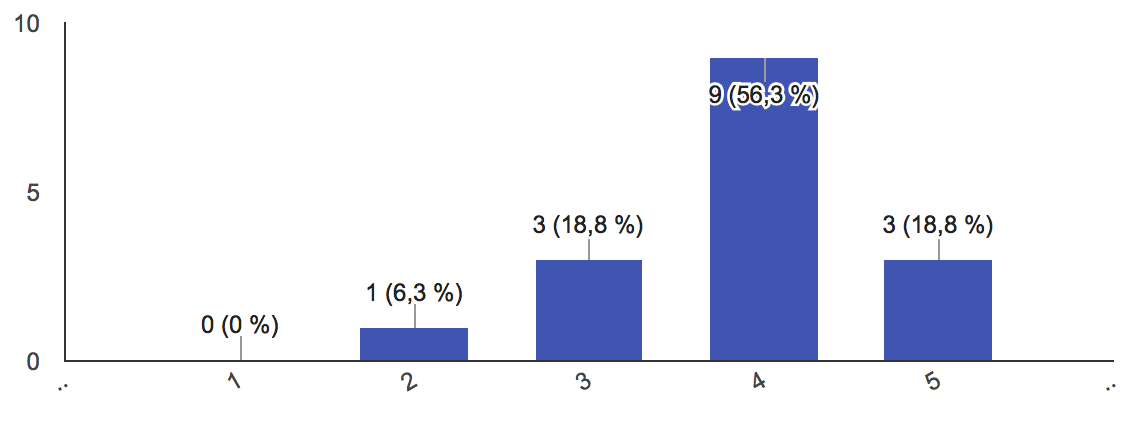
\includegraphics[width=7cm]{figures/overall_evaluation/q10_the_cluster_was_a_fun_and_playful_way_of_learning_the_concepts} }}
    \label{fig:eval_motivation}%
\end{figure}

\begin{figure}[H]
    \centering
    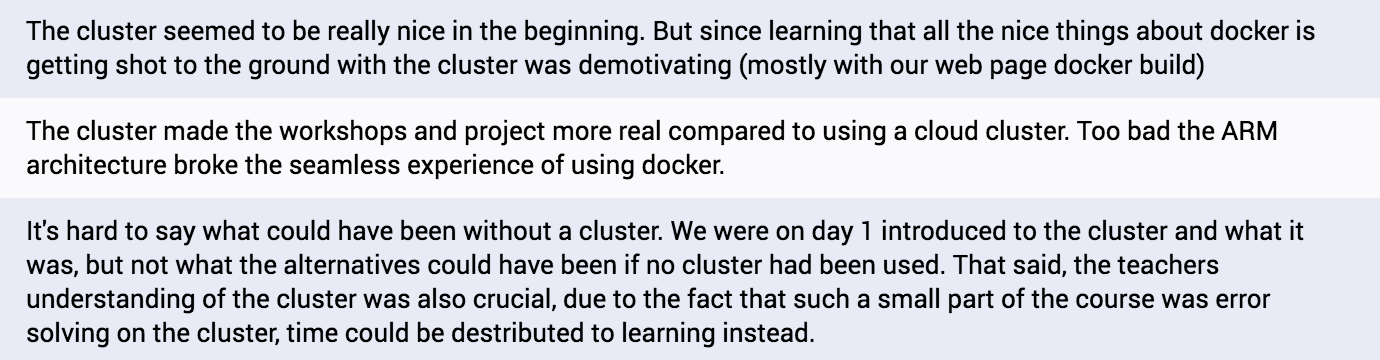
\includegraphics[width=\textwidth]{figures/overall_evaluation/comments_motivation}
\end{figure}


\subsection*{Relation to the real world}


\begin{figure}[H]%
    \centering
    \subfloat[Using a cloud provider (e.g. Google Container Engine) instead of a hands-on tool would have improved my learning]{{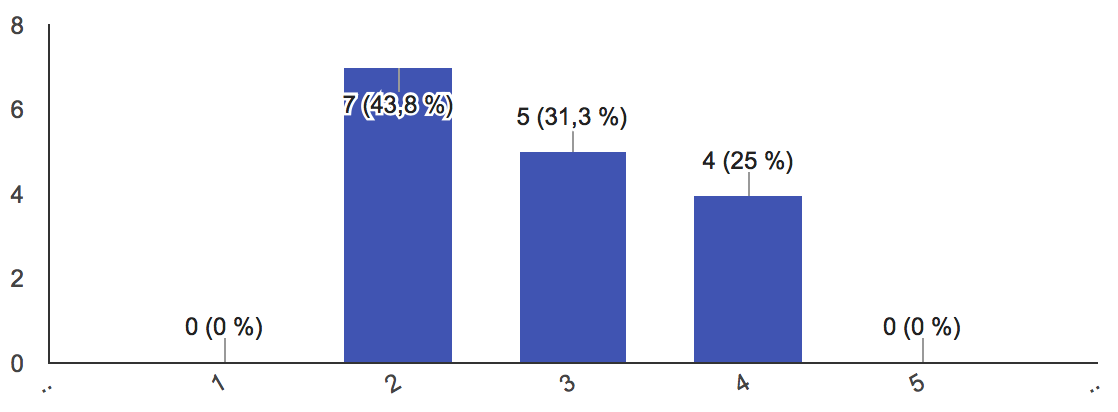
\includegraphics[width=7cm]{figures/overall_evaluation/q11_using_a_cloud_provider_instead_of_a_hands-on_tool_would_have_improved_my_learning} }}%
      \qquad
    \subfloat[The cluster represents a small-scale datacenter]{{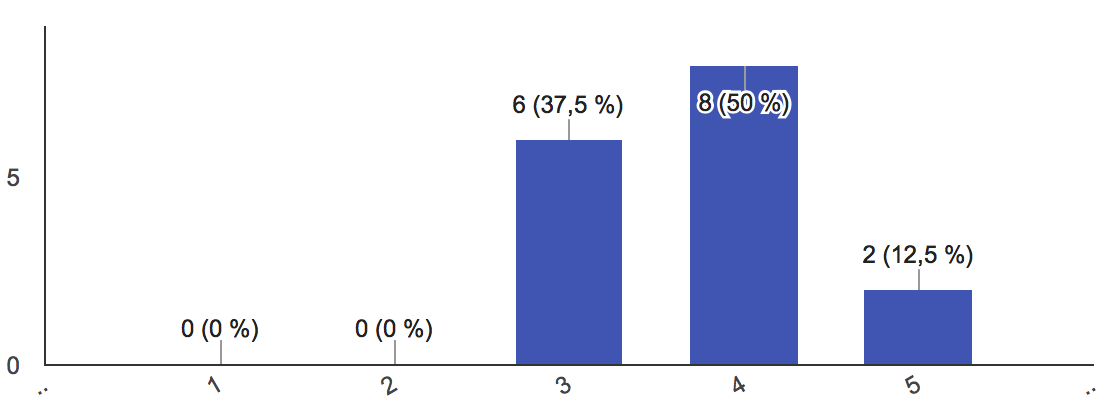
\includegraphics[width=7cm]{figures/overall_evaluation/q12_the_cluster_represents_a_small-scale_datacenter} }}%
    \qquad
    \subfloat[The cluster improved my skills in relevant technologies]{{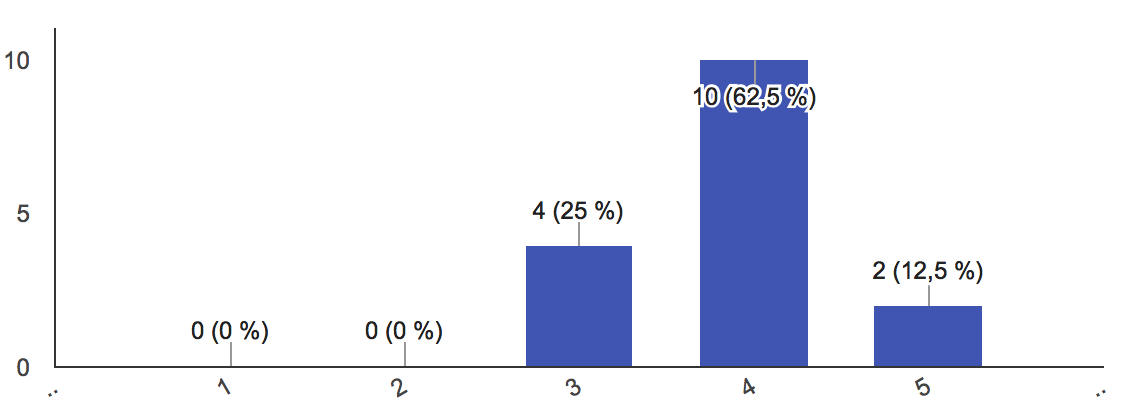
\includegraphics[width=7cm]{figures/overall_evaluation/q13_the_cluster_improved_my_skills_in_relevant_technologies} }}
    \label{fig:eval_real_world}%
\end{figure}

\begin{figure}[H]
    \centering
    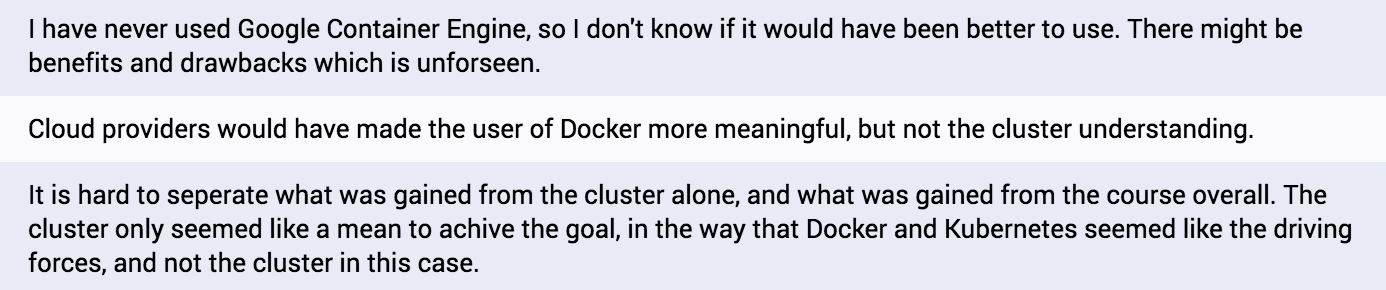
\includegraphics[width=\textwidth]{figures/overall_evaluation/comments_real_world}
\end{figure}

\section*{Evaluation of the learning activity}
The second part of the questionnaire consisted of questions about the designed learning activity.

\subsection*{Course structure}
\begin{figure}[H]%
    \centering
    \subfloat[The distribution of theory and practical work was suitable]{{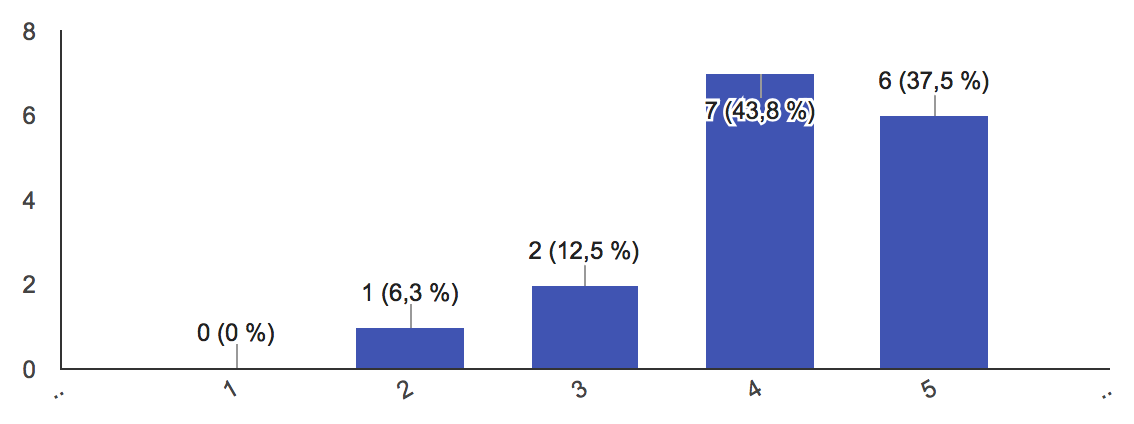
\includegraphics[width=7cm]{figures/overall_evaluation/q14_the_distribution_of_theory_and_practical_work_was_suitable} }}%
      \qquad
    \subfloat[The order of the topics was well-planned]{{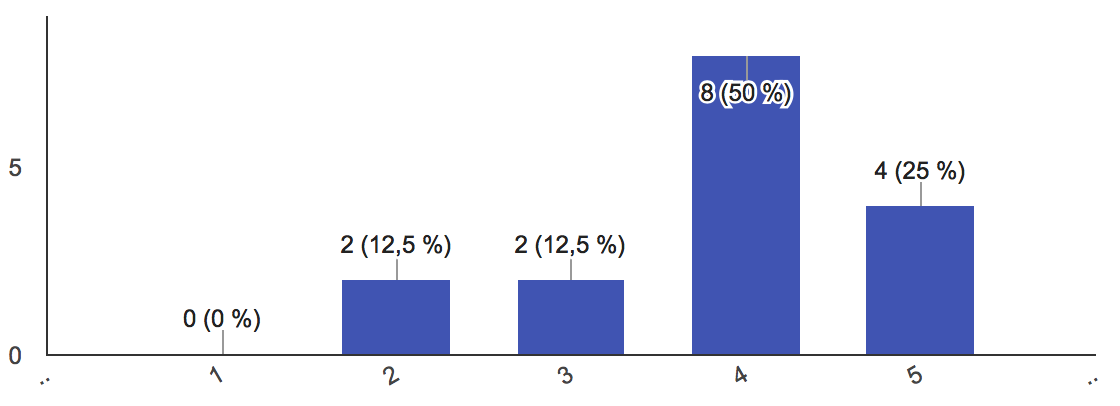
\includegraphics[width=7cm]{figures/overall_evaluation/q15_the_order_of_the_topics_was_well-planned} }}%
    \qquad
    \subfloat[The problem based project allowed me to apply the concepts and theories]{{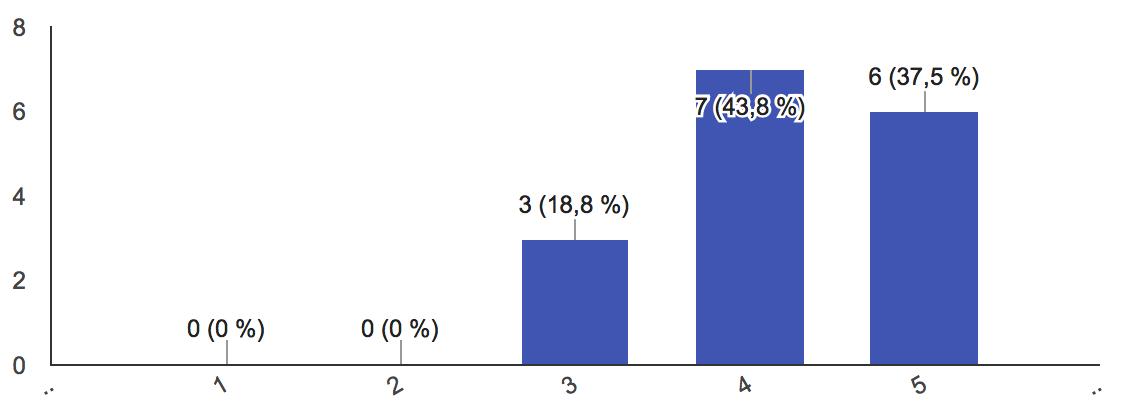
\includegraphics[width=7cm]{figures/overall_evaluation/q16_the_problem_based_project_allowed_me_to_apply_the_concepts_and_theories} }}
          \qquad
    \subfloat[The workshops provided me with the necessary skills for the project work]{{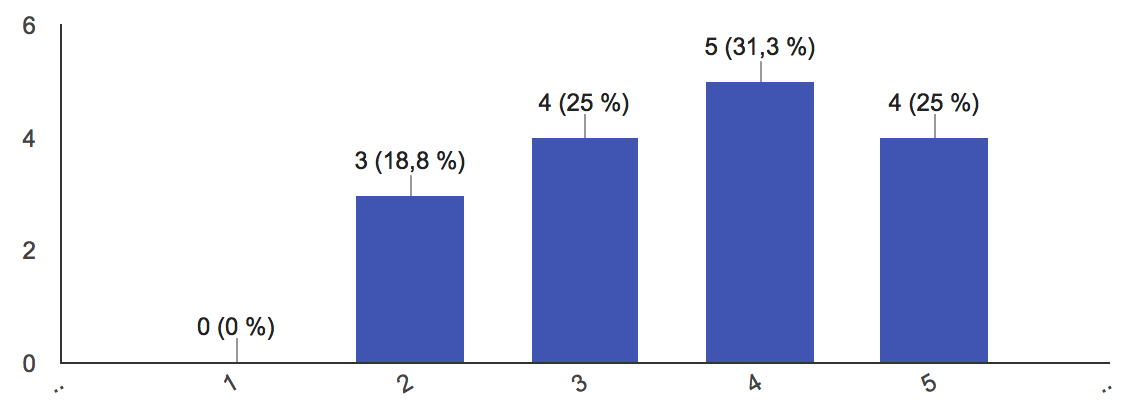
\includegraphics[width=7cm]{figures/overall_evaluation/q17_the_workshops_provided_me_with_the_necessary_skills_for_the_project_work} }}%
    \label{fig:eval_course_structure}%

\end{figure}

\newpage

\begin{figure}[H]
    \centering
    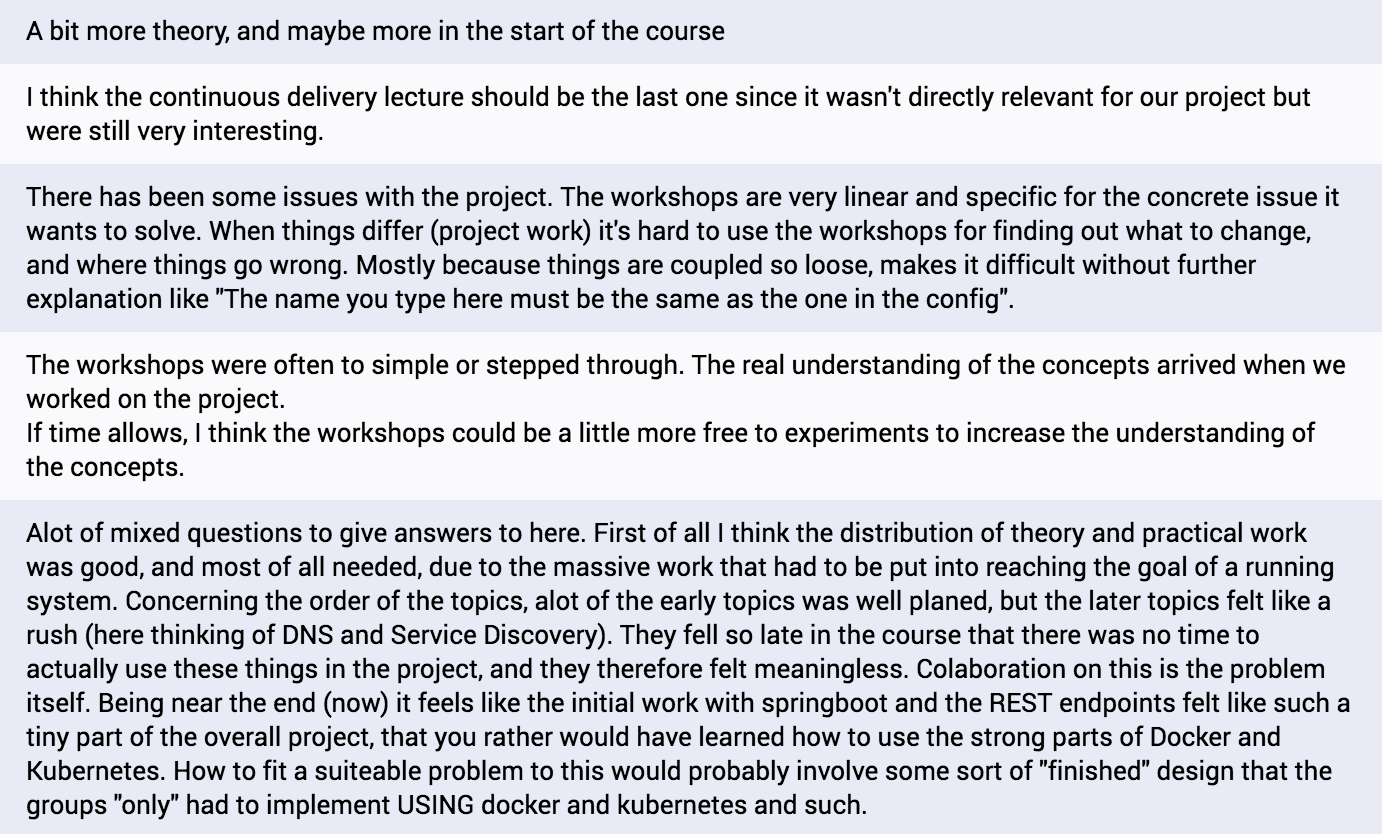
\includegraphics[width=\textwidth]{figures/overall_evaluation/comments_course_structure}
\end{figure}

\subsection*{Materials}
\begin{figure}[H]%
    \centering
    \subfloat[The reading and video materials provided me with the essentials for each module]{{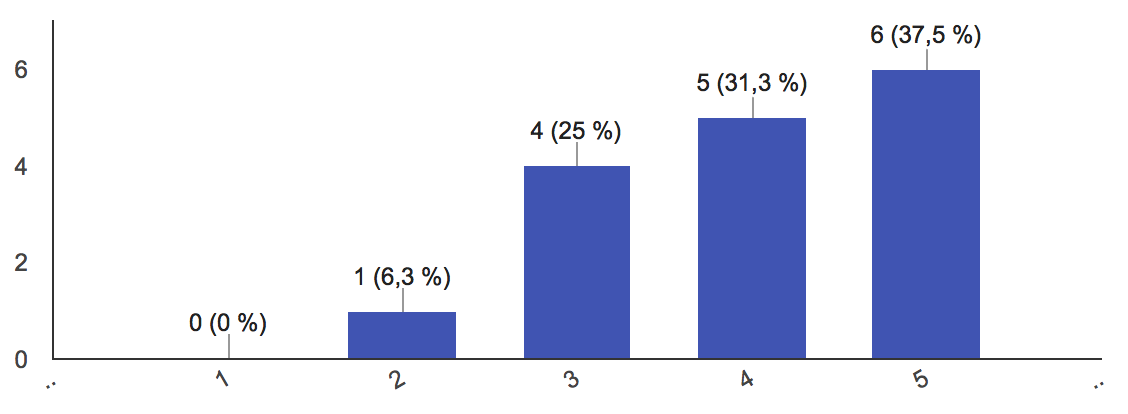
\includegraphics[width=7cm]{figures/overall_evaluation/q18_the_reading_and_video_materials_provided_me_with_the_essentials_for_each_module} }}%
      \qquad
    \subfloat[The slides covered the necessary theory]{{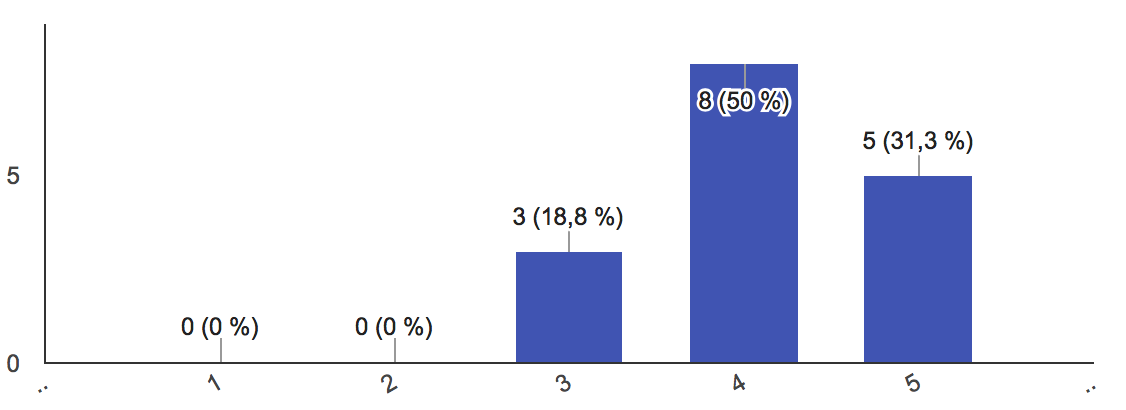
\includegraphics[width=7cm]{figures/overall_evaluation/q19_the_slides_covered_the_necessary_theory} }}%
    \qquad
    \subfloat[The blog (rpi-cloud.com) helped me getting started with Spring Boot and Spring Cloud]{{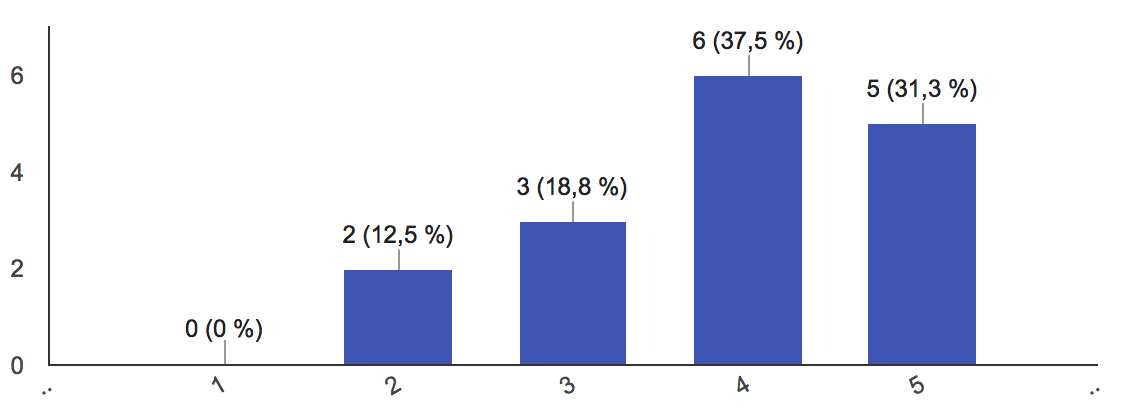
\includegraphics[width=7cm]{figures/overall_evaluation/q20_the_blog_helped_me_getting_started_with_Spring_Boot_and_Spring_Cloud} }}
    \label{fig:eval_materials}%
\end{figure}


\begin{figure}[H]
    \centering
    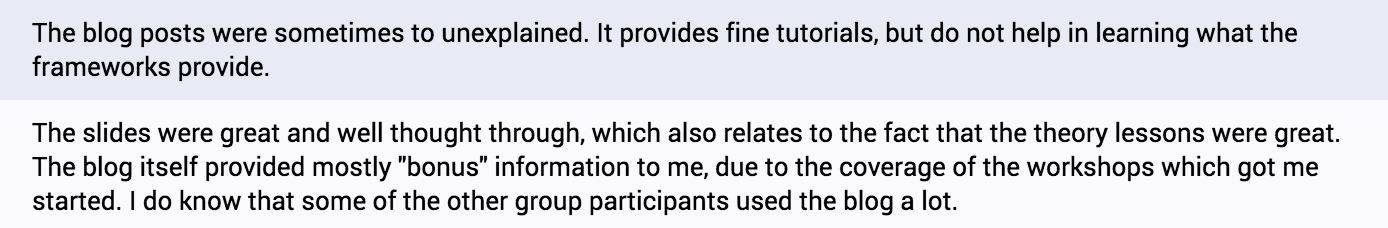
\includegraphics[width=\textwidth]{figures/overall_evaluation/comments_materials}
\end{figure}

\subsection*{Comparison}
\begin{figure}[H]%
    \centering
    \subfloat[In comparison with other courses my overall rating of the course is]{{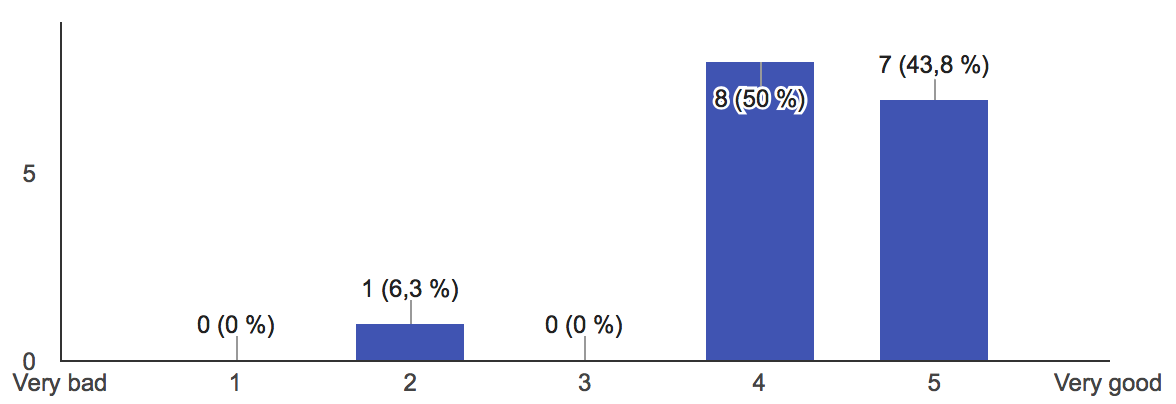
\includegraphics[width=7cm]{figures/overall_evaluation/q21_in_comparison_with_other_courses_my_overall_rating_of_the_course_is} }}%
    \label{fig:eval_overall_rating}%
\end{figure}

\begin{figure}[H]
    \centering
    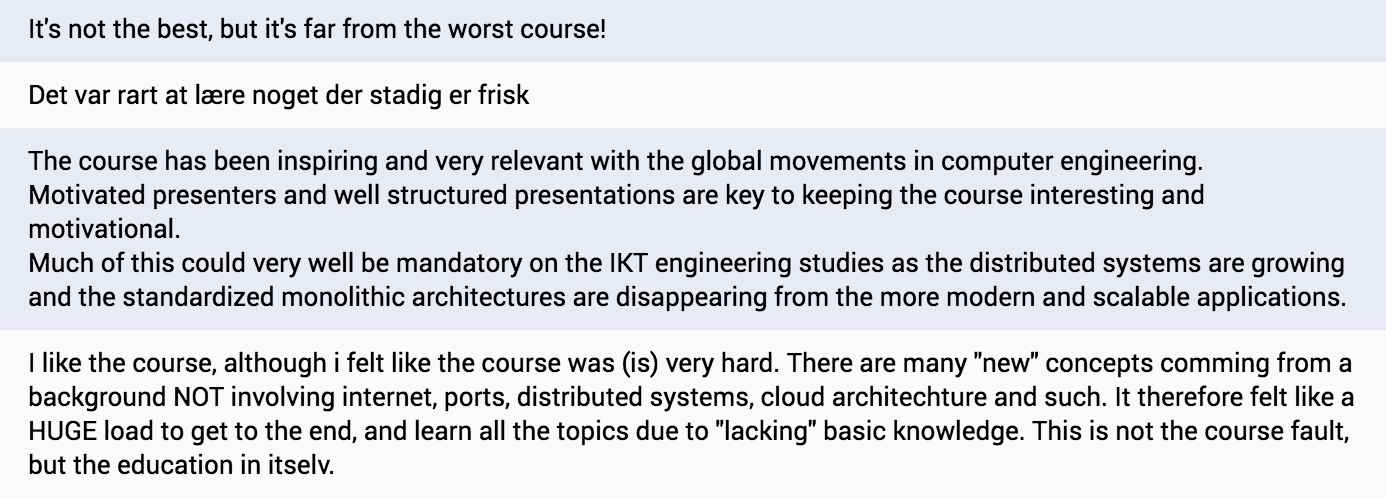
\includegraphics[width=\textwidth]{figures/overall_evaluation/comments_comparison}
\end{figure}
